\section{A methodology for the study of feedback-loop systems in Edge Computing}\label{summary:methodology}

\begin{figure}
    \centering
    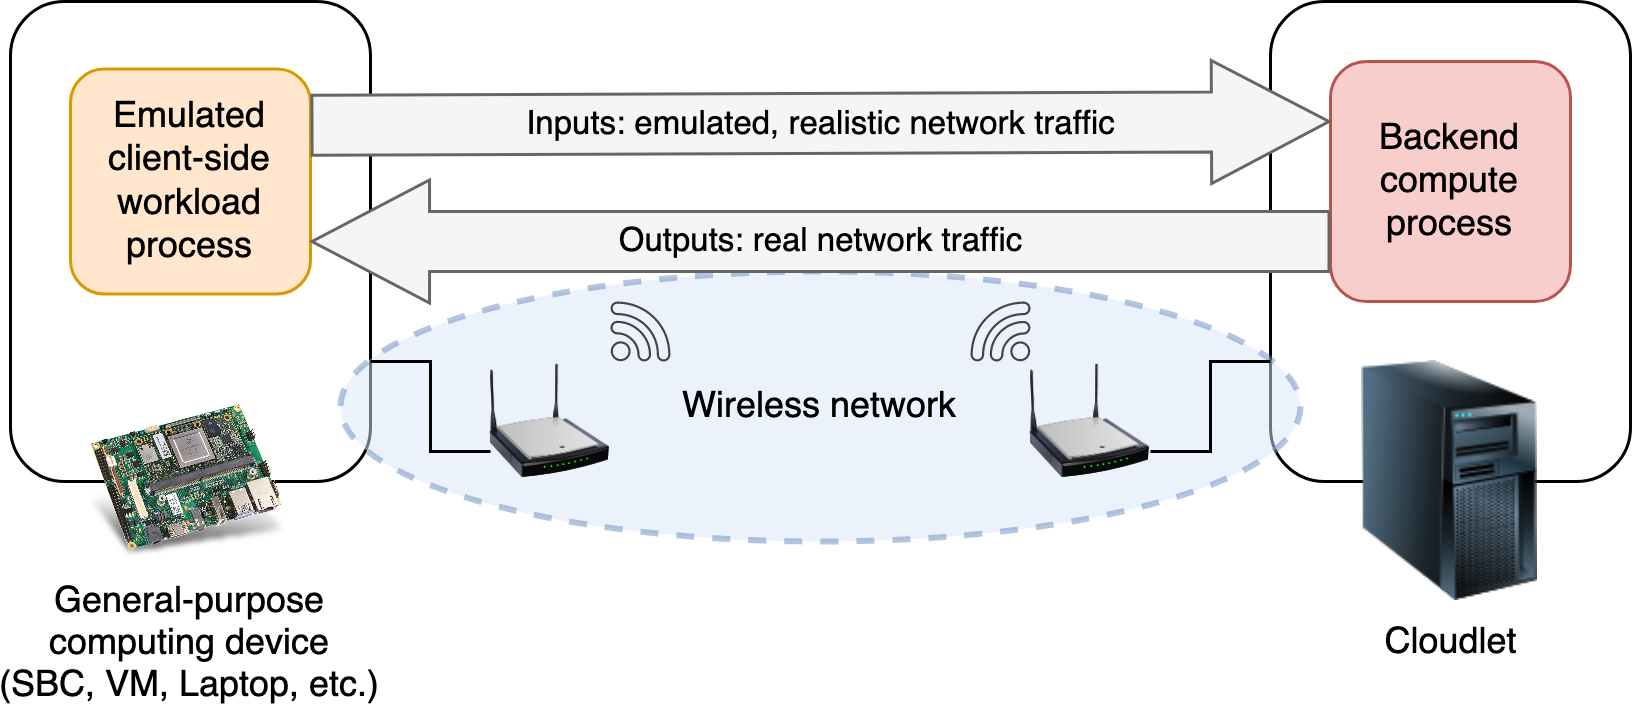
\includegraphics[width=.8\textwidth]{Figs/methodology.png}
    \caption{%
        Overview of the proposed methodology for the study of feedback-loop systems on edge computing infrastructure.
        The  client side of the system is replaced with an emulation executed on a general-purpose computing device.
        The backend/server side of the system along with the network remain unchanged.
    }\label{fig:methodology}
\end{figure}

As discussed above, benchmarking infrastructures for edge-bound applications featuring feedback-loops is challenging, in particular when dealing with applications with high sensitivity to latency (such as \ac{NCS}) or with human involvement (such as \ac{WCA}).
In the following, we introduce our methodological framework for tackling this challenge.

A general overview of our methodology is illustrated in \cref{fig:methodology}.
It is based on the core idea of executing an emulation of the target workload on top of the real hardware on which it is to be deployed.
We replace the client side of the system with a realistic emulation of the desired behaviors; this emulation is implemented in software deployed on \ac{COTS} general-purpose computing devices.
The backend side and the network are not changed.

Two main arguments drive this approach.
One, the difficulty of scaling the number of clients in these systems in a research context.
The systems we target exhibit a centralized nature in which a potentially large number of clients offload computation to a single central compute node.
The client-side component of the applications of interest for this research is often complex to scale, either due to the involvement of humans (as in the case of \ac{WCA}) or due its cyber-physical nature (in \acp{NCS}).
Emulating this component reduces this complexity by moving it into the software domain, allowing for easier scaling through the use of cheap, general-purpose hardware such as single-board computers (e.g. Raspberry Pis, Beaglebones, etc.).

And two, it maintains the realism of the most complex parts of the system.

\todo[inline]{Fix and finish}

In the following, we will discuss the initial implementation of this methodology to two different classes of applications.
We first discuss the methodology in the context of a human-in-the-loop application, \acl{WCA}, in section \cref{ssec:methodology:wca}.
Then, in \cref{ssec:methodology:ncs}, we present an exploration into it's utility for the study of \acf{NCS}.


\subsection{Applying the methodology to \acs{WCA}}\label{ssec:methodology:wca}

\begin{figure}
    \centering
    \begin{subfigure}[b]{.47\textwidth}
        \centering
        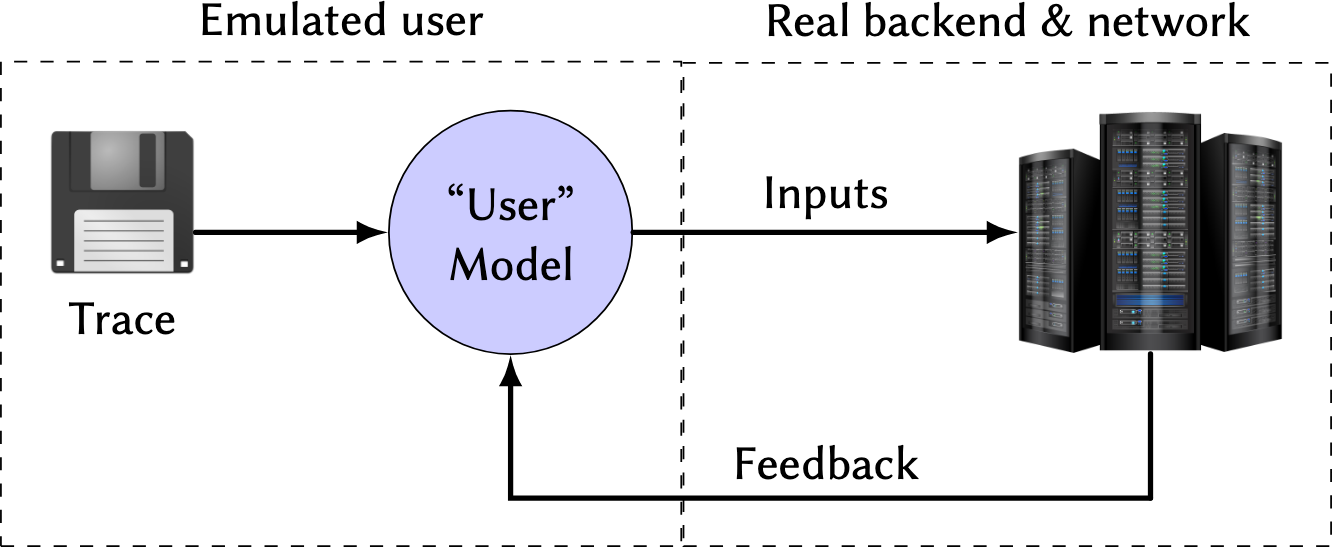
\includegraphics[width=\textwidth]{Figs/trace_edgedroid.png}
        \caption{%
            High level conceptual design of our methodology for \ac{WCA}.
            We replace the human by a trace-driven emulation.
            This allows us to maintain realism in inputs sent over the network to the compute process on the backend, while simplifying the design of the client software.
        }
    \end{subfigure}
    \hfill
    \begin{subfigure}[b]{.47\textwidth}
        \centering
        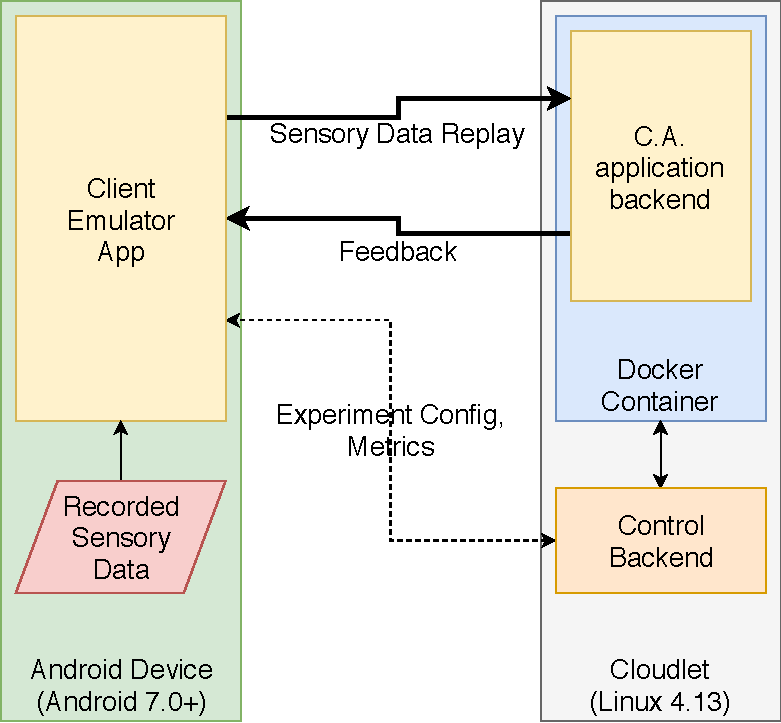
\includegraphics[width=\textwidth]{publications/2018DemoScalingOnTheEdge/img/TraceReplay_GenArch}
        \caption{%
            Architectural overview of the EdgeDroid \num{1.0} tool.
            The ``client emulator app'' implements the aforementioned user model together with the required networking functionality to connect to a \ac{WCA} backend running on a cloudlet.%
        }
    \end{subfigure}\\
    \medskip
    \begin{subfigure}[t]{\textwidth}
        \centering
        \adjustbox{scale=0.7}{
            \begin{tikzpicture}[align=center,
                node distance=.5cm and 1.5cm,
                every initial by arrow/.style={-{Latex[length=2mm]}}]
                % Place nodes
                \node [initial, state, minimum size=6em, initial text=] (play) {Play};
                \node [state, above right=of play, minimum size=6em] (change) {Change\\step};
                \node [state, below right=of play, minimum size=6em] (rewind) {Rewind};
                \node [state, accepting, above right=of rewind, minimum size=6em] (shutdown) {Shutdown};

                % Draw edges
                \path[draw, -{Latex[length=2mm]}]
                (play) edge [bend right=20] node[left] {Step done} (rewind)
                edge [bend left=20] node[left] {Got feedback\\(\emph{positive})} (change)
                edge [out=140,in=220,looseness=6] node[left] {Step\\not done} (play)

                (change) edge [bend left=20] node[right] {Step changed} (play)
                edge [bend left=20] node[right] {All steps done} (shutdown)

                (rewind) edge [bend right=20] node[right] {Rewound} (play)
                edge [bend right=20] node[right] {Too many rewinds} (shutdown);

            \end{tikzpicture}
        }
        \caption{State diagram of the user model governing the replay of the pre-recorded trace at runtime. This model approximates the behavior of an ``ideal'' human, one that is patient and makes no mistakes.}\label{fig:usermodel}
    \end{subfigure}
    \caption{%
        Overview of our first implementation of the methodology for \ac{WCA}.
    }\label{fig:edgedroid1:trace}
\end{figure}

We first introduce our methodology in \cref{paper:olguinmunoz2018demoscaling,paper:olguinmunoz2019edgedroid}.
The former corresponds to an extended abstract paper which discusses a high level overview of our approach; the latter presents a deeper, more complete discussion about the implementation together with some first experimental results.

The overall goal of these papers is to explore this methodological approach as applied to \ac{WCA}.
As discussed in \cref{chap:introduction}, the main challenge to benchmarking \ac{WCA} --- and other ``human-in-the-loop'' applications on the edge --- concerns the involvement of human beings in their operation.
Humans are unreliable, and, perhaps more importantly, hard to scale.
\todo[inline]{More reasons}

The implementation of the client-side emulation necessary for our methodology follows in these works a trace-based design.
We introduce a tool, \emph{EdgeDroid \num{1.0}}, which replays a pre-recorded trace of sensory inputs to the original \ac{WCA} backend.
The tool is implemented in Android, allowing for its easy deployment on the same kind of \ac{COTS} mobile devices on which real \ac{WCA} applications are intended to run in the future.
Furthermore, this tool is instrumented, allowing us to collected a multitude of system-level metrics at runtime which can then be analyzed.
On the other hand, the trace in question corresponds to a pre-recorded sequence of sensory inputs obtained from a real execution of the \ac{WCA} by a human volunteer.
The trace is recorded in a near-ideal setting, such that it does not include either human mistakes or segments with degraded system responsiveness.
Once recorded, the trace is manually segmented into the logical component steps of the task, and these are replayed in sequence back to the backend by the EdgeDroid tool.

We opt for a trace-based approach for our first implementation of the methodology for \ac{WCA} for three key reasons.
The first of these is the level of realism if affords in terms of the payloads sent over the network and, in particular, processed by the backend.
Using a trace ensures that the same computation is performed on the edge as if a human was involved, while also ensuring a reproducible application execution path.

The second is simplicity, as such an approach does not require complex modeling of human behavioral patterns, merely the observation and recording of them.
Compatible traces can be easily obtained simply by instrumenting existing \ac{WCA} client applications to record all captured inputs.

The final advantage corresponds to extensibility.
As long as the tasks belong to the same category of \ac{WCA} applications (in this case, step-based cognitive assistance), using a trace makes extending the tool to different tasks merely a matter of recording a new trace.

\todo[]{}



reproducible and comparable workload, we use a trace-based design for the client-side emulation.
.

To then use the trace for reproducible experiments, we introduce a benchmarking suite which can replay the trace to the original application.
This results in the same computation to be performed on the edge as if a human was involved, while also ensuring a reproducible application execution path.
Additionally, the suite is instrumented to collect system level metrics at runtime for posterior analysis.

However, merely replaying the trace is not enough, as disparities between system responsiveness at recording versus replay time can cause the trace so drift out of synchronization with the current state of the system.
Thus, we introduce here the concept of a human user model which is able to adapt its behavior in a realistic manner based on the current responsiveness of the system by systematically controlling the replay of the trace.
The initial approximation we introduce, illustrated in \cref{fig:usermodel}, here is that of a human that is patient and does not make mistakes, and any error message received from the application backend is ignored.
The trace is preprocessed into segments that correspond to individual steps of the \ac{WCA} application; this is performed manually as a preparation step.
The user model then replays each segment in order; whenever feedback corresponding to a change of step is received from the \ac{WCA} backend, the user model transitions to the next segment in the trace, no matter whether the current segment has been replayed out completely or not.
On the other hand, if no step transition feedback has been received at the end of the current trace segment, the model rewinds the trace a $\tau$ seconds and tries again.
To avoid infinite loops, where the application is stuck on a step forever, we have a maximum number of possible rewinds, after which the application shuts down.

\todo[inline]{EdgeDroid paper}



\begin{figure}
    \centering%
    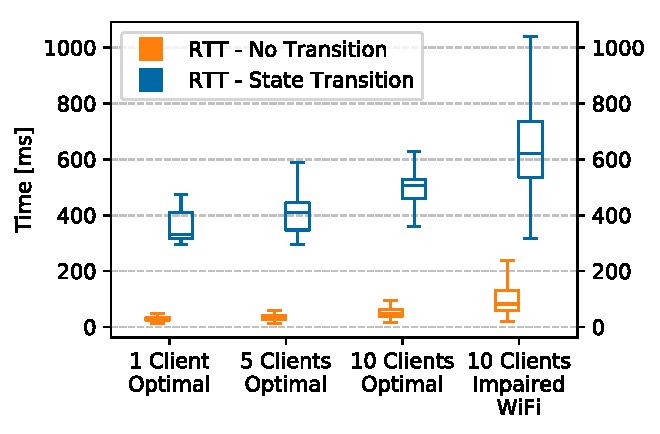
\includegraphics[width=.85\textwidth]{publications/2019EdgeDroid/plots/comparison/nofonts/rtt_fb_vs_nofb}%
    \caption{Comparison of round-trip-times for inputs that triggered a state transition in the task model versus inputs that did not.}%
    \label{fig:comparison:rtt}%
\end{figure}%
\begin{figure}
    \centering%
    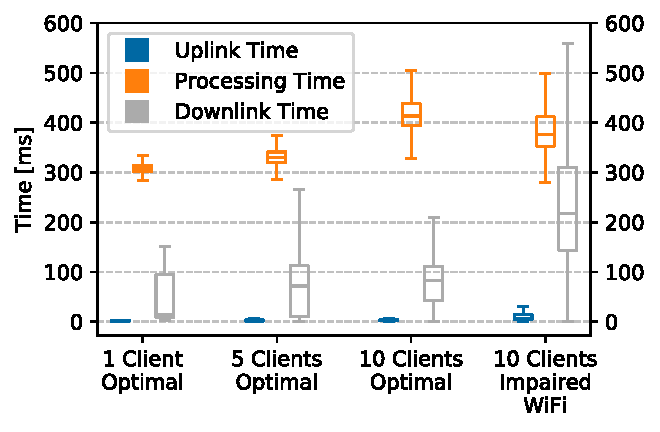
\includegraphics[width=.85\textwidth]{publications/2019EdgeDroid/plots/comparison/nofonts/box_feedback}%
    \caption{Distribution of latency across system components for inputs that triggered a state transition in the task model.}%
    \label{fig:comparison:feedback}%
\end{figure}%
\begin{figure}%
    \centering%
    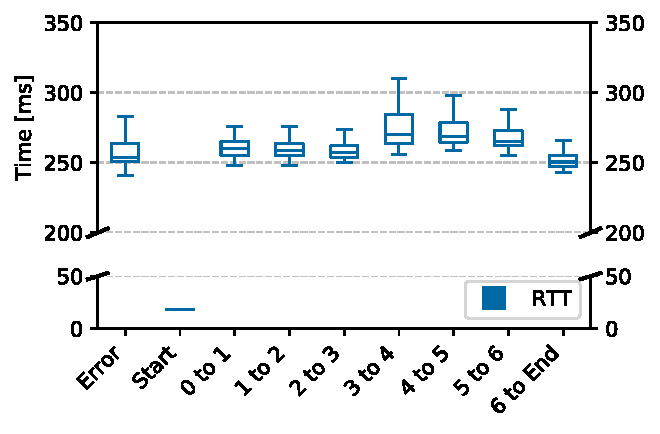
\includegraphics[width=.85\textwidth]{publications/2019EdgeDroid/plots/comparison/nofonts/box_taskstep}%
    \caption{Round-trip-times for input-feedback cycles associated with state transitions in the internal task model for a single client connected over an optimal wireless link.}%
    \label{fig:comparison:tasksteps}
\end{figure}%

The goal of this paper is to provide a methodological approach to studying these latency trade-offs, along with a tool, EdgeDroid 1.0\footnote{We plan to make the EdgeDroid 1.0 benchmarking suite available as Free and Open Source Software and the recorded traces under a Creative Commons License.}, that simplifies the benchmarking of human-in-the-loop applications.
We view EdgeDroid 1.0 to be the very first, and simplest, of a family of tools that will embody increasingly sophisticated and accurate models of user behavior.

Due to the complex nature of the applications and the infrastructure, we opt for experimentally studying the trade-offs in a repeatable and controllable fashion.
This is difficult mainly due to the unpredictable reaction of human users to the feedback from the backend --- a user might very well misinterpret the feedback handed to them.
EdgeDroid 1.0 mimics the operation of human-in-the-loop applications by replaying recorded traces of sensory input.
This sensory information is then processed by the original compute process at the backend, generating feedback.
However, this feedback is not processed by humans, but by a parameterizable model of human reaction.
Through synchronized time tracking at the different processing points of the application, EdgeDroid 1.0 allows for accurate measurements of key performance metrics such as the distribution of delays across the application pipeline.
Analysis of these metrics can be performed down to the individual input sample, allowing us to zoom into the internal model of the application under consideration.
Thus, EdgeDroid 1.0 allows us to illuminate the many latency trade-offs existing at the level of the infrastructure, as well as the level of the application.
It can also be used for debugging and validation, by comparing the expected execution flow of a particular trace with the actual flow during the benchmarking.
To the best of our knowledge, this experimentally-driven benchmarking approach is the first one towards experimental performance characterization and potential optimization of human-in-the-loop applications

\Cref{fig:comparison:rtt} presents a comparison of the total measured round-trip-times (RTTs) both for inputs which caused a state transition and inputs that did not.
Next, \cref{fig:comparison:feedback} shows a comparison of the distribution of latencies across system components for inputs that caused an internal state change in the task model of the application.
We differentiate according to the three main components contributing to latency, namely \emph{uplink} and \emph{downlink transmissions}, and \emph{backend processing}.
Finally, \cref{fig:comparison:tasksteps} depicts the distribution of RTTs for each transition in the internal task model for a single client connected over an optimal wireless link.
These metrics were calculated by recording the measured input-feedback cycle delay corresponding to a change in state within the application.
Thus, for instance, the measurements located at column ``3 to 4'' in the figure correspond to the aggregated round-trip-times for every input-feedback cycle corresponding to a change from state 3 to state 4 within the application task model, for the 100 repetitions of the scenario.

In the following discussion we will refer to inputs which triggered a transition in the task model as \emph{feedback-rich inputs} and those that did not as \emph{feedback-less inputs}.

For the analysis of these results, we will take into consideration the bound of \SI{600}{\milli\second} response time for step-by-step task-guidance derived by the authors of~\cite{Chen:AnEmpiricalStudyOfLatency}.
This bound marks the point after which further delays in the delivery of feedback to the user start to negatively affect user experience, and allows for a straightforward evaluation of the responsiveness of the system.

We will begin our analysis of the experiment results with \Cref{fig:comparison:rtt}.
These results present a stark contrast in the round-trip-times for inputs which cause a state transition versus inputs that do not, with RTTs for the former being up to an order of magnitude greater.
It's worth mentioning though that responses to feedback-less inputs are invisible to the user, and are just included here as a sort of baseline to compare feedback-rich round-trip times with.

We can identify a pair of interesting effects in the scaling of the task-guidance WCA application.
One, scaling behavior for the application seems to be linear with respect to the number of clients.
Two, in the case of the impaired WiFi, the effect on the feedback-rich inputs is very pronounced, with the average of the RTTs for these inputs being over the previously discussed bound of \SI{600}{\milli\second}.

It is worth noting that already at just 10 clients the response times for feedback-rich inputs are very close to the bound.
Looking at this through the lens of a an application developer, it could hint at a need for optimization of the later parts of the application pipeline, since RTTs for inputs which are discarded in the detection stage of the pipeline (i.e.\ feedback-less inputs) are still well below \SI{200}{\milli\second}.

EdgeDroid 1.0 allows researchers to zoom into specific components of the application feedback loop, as exemplified by \cref{fig:comparison:feedback}.
From this figure it is clear that the main component which contributes to latency in the optimal case is the backend processing, further lending credibility to our previous comment on the need for optimization.
Nevertheless, when the link quality decreases, the delays on the downlink start to overshadow the delays on the processing.
Here, the downlink time sometimes almost reaches the ideal bound by itself.
A system designer might then conclude from this that in order to be able to scale the application, their focus needs to be on improving the quality of the wireless link before increasing the processing power on the backend.

Finally, EdgeDroid 1.0 allows even more insights to be gained by homing in to individual steps in a task-guidance WCA. Consider \cref{fig:comparison:tasksteps}.
The figure shows clears spikes in latencies at the transitions from task state 3 to 4 and from task state 4 to 5, which could indicate to the application developer that these specific transitions are ripe for optimization.


\todo[inline]{\cref{paper:olguinmunoz2019edgedroid}}\label{summary:2019edgedroid}

\subsection{Applying the methodology to \acsp{NCS}}\label{ssec:methodology:ncs}

\todo[inline]{\Cref{paper:olguinmunoz2022cleave} implements both the methodology and the tool.}

\begin{figure*}
    \centering
    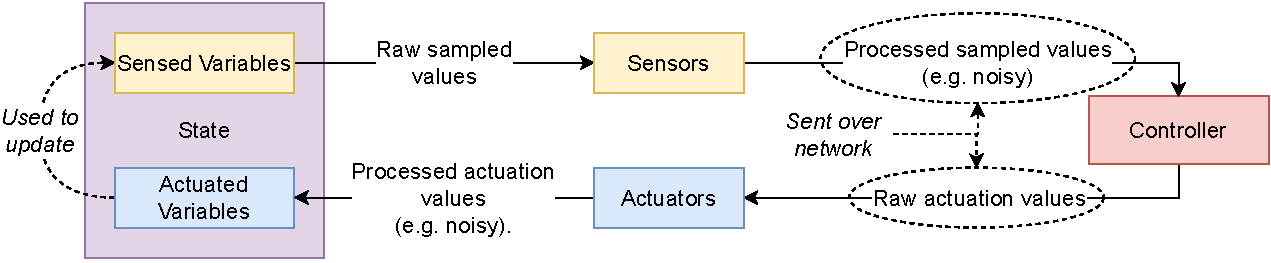
\includegraphics[width=.8\textwidth]{publications/2022CLEAVE/images/CLEAVE_NCS_structure}
    \caption{
        Structure of an emulated \acl*{NCS} in \acs*{CLEAVE}.
    }\label{fig:cleave:ncs:struct}
\end{figure*}

We overcome this issue by proposing a completely virtual plant allowing for unparalleled flexibility in changing the plant model and characteristic features of the experiments.
In this paper, we present the first fully-software-based framework for scalable and repeatable benchmarking of edge-native \ac{NCS}.
As edge computing begins being adopted by industry, more and more variations have begun to appear in literature.
``Near'', ``far'', ``core'', and ``telco'' edge describe variations of the original concept and are becoming ubiquitous in new research.
While the core idea of edge computing is widely accepted as fundamental for pervasive \acp{NCS} in general, understanding the strengths and weaknesses of such different edge concepts is of paramount importance.

Our framework, \ac{CLEAVE}, aims to simplify the repeatable and scalable benchmarking of such systems.
It is fully virtualized, inspired by our previous work on benchmarking human-in-the-loop applications on the edge~\cite{Olguin2019EdgeDroid}.
The tool consists of a benchmarking framework and software development kit for the development of emulated physical systems and softwarized controllers.
These virtual \acp{NCS} can then be deployed on real networks for reparametrizable, repeatable, and reproducible benchmarking of the complete system.

\ac{CLEAVE} is built using \emph{Python 3.8}, making it highly extensible and able to harness the multitude of already existing user libraries.
It is furthermore compatible with container technologies such as \emph{Docker}\footnote{Docker Engine: \url{https://www.docker.com/}}, making it suitable for automated deployment, scaling, and benchmarking on industry-standard edge setups using container orchestration solutions.

In this work, we aimed to tackle this issue through a fully software-based framework for repeatable, reproducible, and easily scalable \ac{NCS} benchmarking with a particular focus on edge deployment.
We argue our approach, \ac{CLEAVE}, embodies a better solution than previous work for a number of reasons:
\begin{enumerate}
    \item Compared to fully physical approaches, such as those used in\ \cite{Baumann2018LowPower} and\ \cite{Cuenca2019UAV}, our approach allows for greater flexibility and scalability.
    The aforementioned approaches rely on specialized and sometimes entirely custom-built physical platforms, and although flexible and cheap approaches such as Zoppi \emph{et al.'s} --- which uses a LEGO-based physical plant --- exist, these still do not reach the level of flexibility afforded by a fully software-based framework.
    Experimenters still need copies of the hardware, making anything other than small-scale setups unfeasible.
    In contrast, our approach requires only general-purpose computing platforms, and can be employed by basically anyone with access to a computer.
    Scalable deployments can in turn easily and cheaply be set up using single-board computers and/or virtual cloud instances.
    \item When compared to simulated approaches such as\ \cite{Ma2019DynamicSched}, \ac{CLEAVE} provides a higher level of realism, in particular with regards to the network segment of the system.
    \item Finally, although it shares much in common with previous emulated approaches such as the one employed in\ \cite{Wang2020VoltageControl}, \ac{CLEAVE} has an advantage by specifically targeting a general-purpose approach using industry-standard, cloud- and edge-native tools and software.
    The tool can easily be deployed and scaled using widely-used frameworks such as Docker Swarm and Kubernetes.
\end{enumerate}

We validate the utility of this tool through an example use case approximating a proposed edge deployment of inverted pendula control loops co-located with video analytics services.
We argue such a use case represents a realistic scenario and appropriate benchmark for the tool, since
\begin{enumerate*}[itemjoin={{; }}, itemjoin*={{; and }}]
    \item the inverted pendulum plant is ubiquitous in \ac{NCS} research
    \item similar setups exist in real-world industrial use
    \item video analytics has long been proposed as a ``killer app'' for edge computing.
\end{enumerate*}
Our results showcase the ability of the framework to extract relevant metrics relating to the stability of the control system, as well as on the performance of the underlying network link.
We believe \ac{CLEAVE} represents an important step towards enabling inexpensive and low-complexity scalable research for real-world deployment of edge-bound \acp{NCS}.

\todo[inline]{Some plots and results}

\begin{figure}
    \centering
    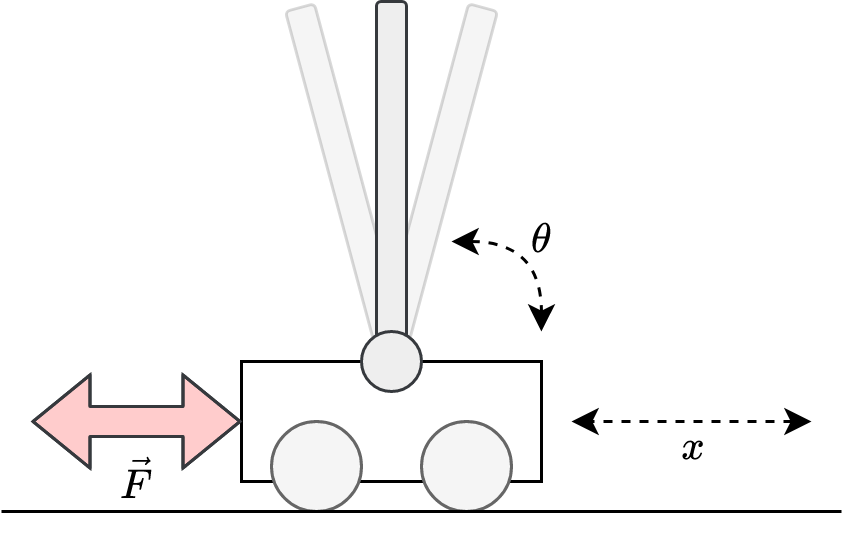
\includegraphics[width=.6\textwidth]{publications/2022CLEAVE/images/inverted_pendulum.png}
    \caption{
        The 2D inverted pendulum system.
    }\label{fig:invpend}
\end{figure}

\begin{figure}[t]
    \centering
    \begin{subfigure}[h]{.22\textwidth}
        \centering
        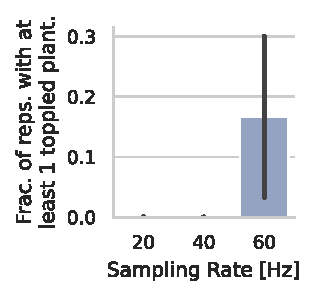
\includegraphics[width=\textwidth]{publications/2022CLEAVE/plots/fixed_video_topple_frac}
        \caption{Toppled plants.}\label{fig:video:toppled}
    \end{subfigure}%
    \hfill%
    \begin{subfigure}[h]{.22\textwidth}
        \centering
        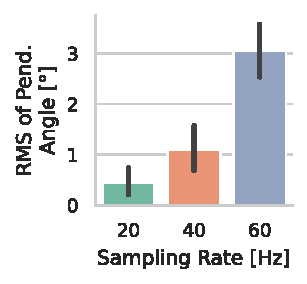
\includegraphics[width=\textwidth]{publications/2022CLEAVE/plots/fixed_video_angle_rms}
        \caption{Angle \ac{RMS}.}\label{fig:video:rms}
    \end{subfigure}\\
    \begin{subfigure}[h]{.22\textwidth}
        \centering
        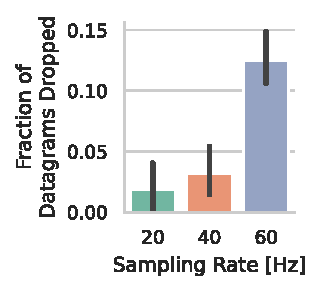
\includegraphics[width=\textwidth]{publications/2022CLEAVE/plots/fixed_video_drop_frac}
        \caption{Packet losses.}\label{fig:video:drop}
    \end{subfigure}%
    \hfill%
    \begin{subfigure}[h]{.22\textwidth}
        \centering
        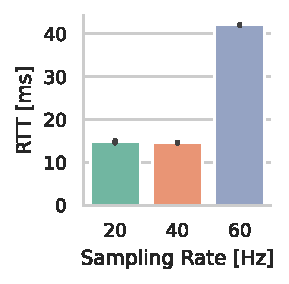
\includegraphics[width=\textwidth]{publications/2022CLEAVE/plots/fixed_video_rtt}
        \caption{\acsp{RTT}.}\label{fig:video:rtt}
    \end{subfigure}%
    \caption{
        Multi-loop, resource-constrained setup results.
        Error bars indicate \SI{95}{\percent} \acp{CI} in all plots.
    }\label{fig:video:results}
\end{figure}

\FloatBarrier%

\subsection{Orchestrating experimentation in edge computing testbeds}

\todo[inline]{\cref{paper:olguinmunoz2022ainur} describes a software framework for testbeds used for the methodology described in this thesis}

In this work, we present our solution to the challenge of testbed automation: Ainur, a framework for wireless testbed automation with a specific focus on end-to-end experimental research in the context of edge-computing using cloud- and edge-native technologies.
Ainur is designed to deploy experimental runs from a workload perspective by configuring the physical testbed, initializing all involved software components, deploying and executing the experimental workload, collecting logs and data, and finally gracefully degrading the system.
The framework allows for dynamic, software-definition of physical and logical links, network topology, cloud and edge computing resources, as well as experimental workload deployment and orchestration.
It heavily leverages cloud-native technologies, such as Docker containers, in order to support a wide variety of different testbed hardware setups and experimental configurations and workloads, as well as to be as easily extendable as possible.
Furthermore, we make Ainur available to the community as \ac{FOSS}.
It can be obtained from the {KTH-EXPECA/Ainur} repository on GitHub~\cite{ainur:github}, released under an Apache version \num{2.0} license.

In this paper, we have introduced a framework for repeatable end-to-end testbed automation in the context of wireless networking and edge computing research.
Named Ainur, it simplifies the execution and verification of end-to-end experimentation by automating the
\begin{enumerate*}[itemjoin={{; }}, itemjoin*={{; and }}]
    \item establishment of physical links between hosts, including the configuration of complex wireless systems such as 4G \ac{LTE} and 5G
    \item provisioning of and connection to remote cloud instances
    \item initialization of \ac{IP} layer connectivity between hosts
    \item collection of logs and data
    \item deployment, scaling, and lifecycle management of containerized processes
\end{enumerate*}.
We have described its general architecture, which follows a layered design mimicking the network stack layers the framework directly interacts with, as well as the underlying assumptions about its deployment environment and specific requirements for its deployment.
We have also outlined a demonstration which showcases the flexibility and power of the framework by deploying two different workloads to our testbed.
We believe our framework represents an important step towards repeatable, replicable, yet low-access barrier end-to-end wireless testbed experimentation.
It has been released as \ac{FOSS} and can be found on GitHub~\cite{ainur:github}.\\

\todo[inline]{Some plots}

\begin{figure}[t]
    \centering
    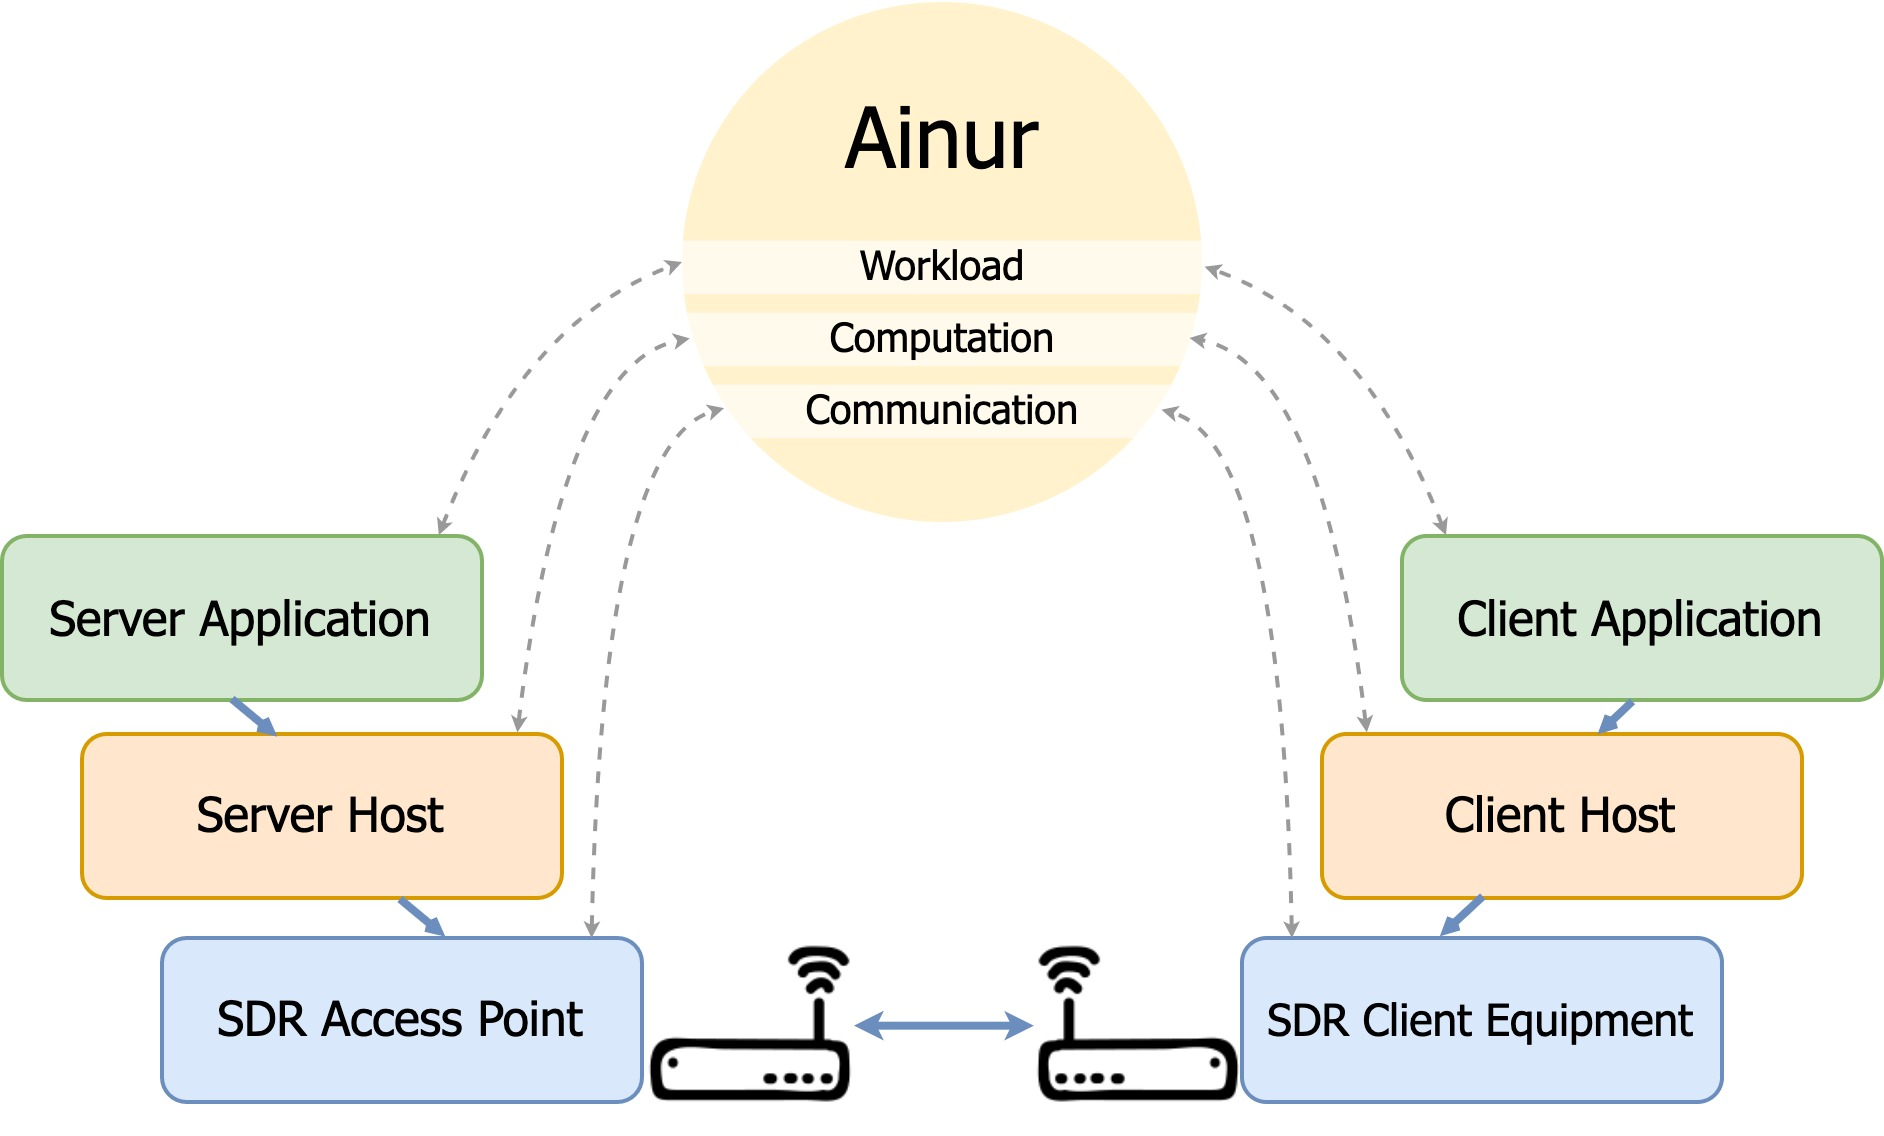
\includegraphics[width=0.9\linewidth]{publications/2022Ainur/figures/overview.jpg}
    \caption{Layered structure of an Ainur experiment}\label{fig:overview}
\end{figure}

\begin{figure*}
    \centering
    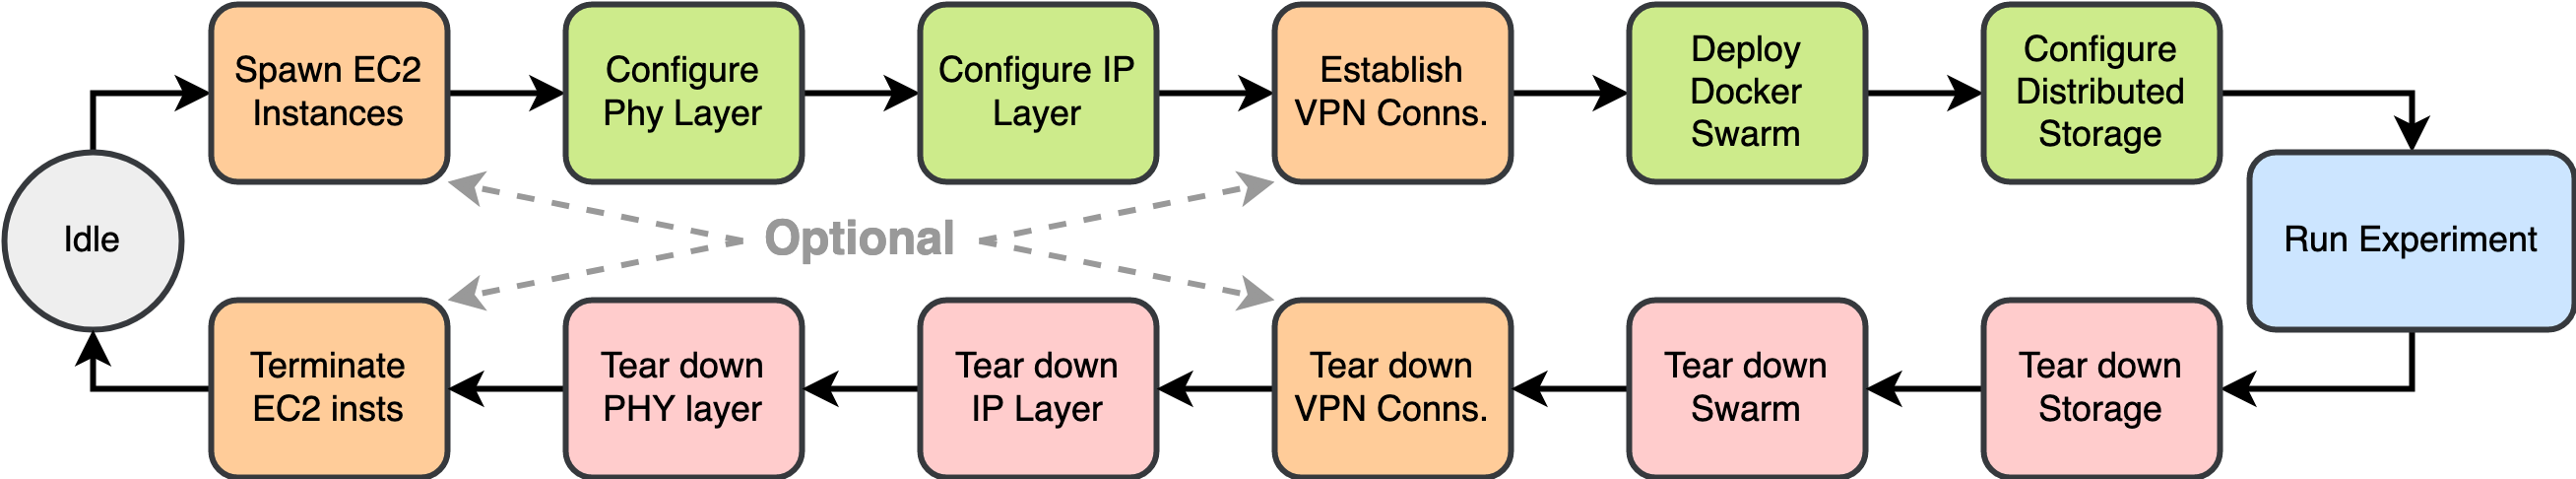
\includegraphics[width=0.8\textwidth]{publications/2022Ainur/figures/flow2.png}
    \caption{Lifecycle of an experimental run in Ainur. Blocks in orange are optional.}\label{fig:flow}
\end{figure*}

\begin{figure*}
    \centering
    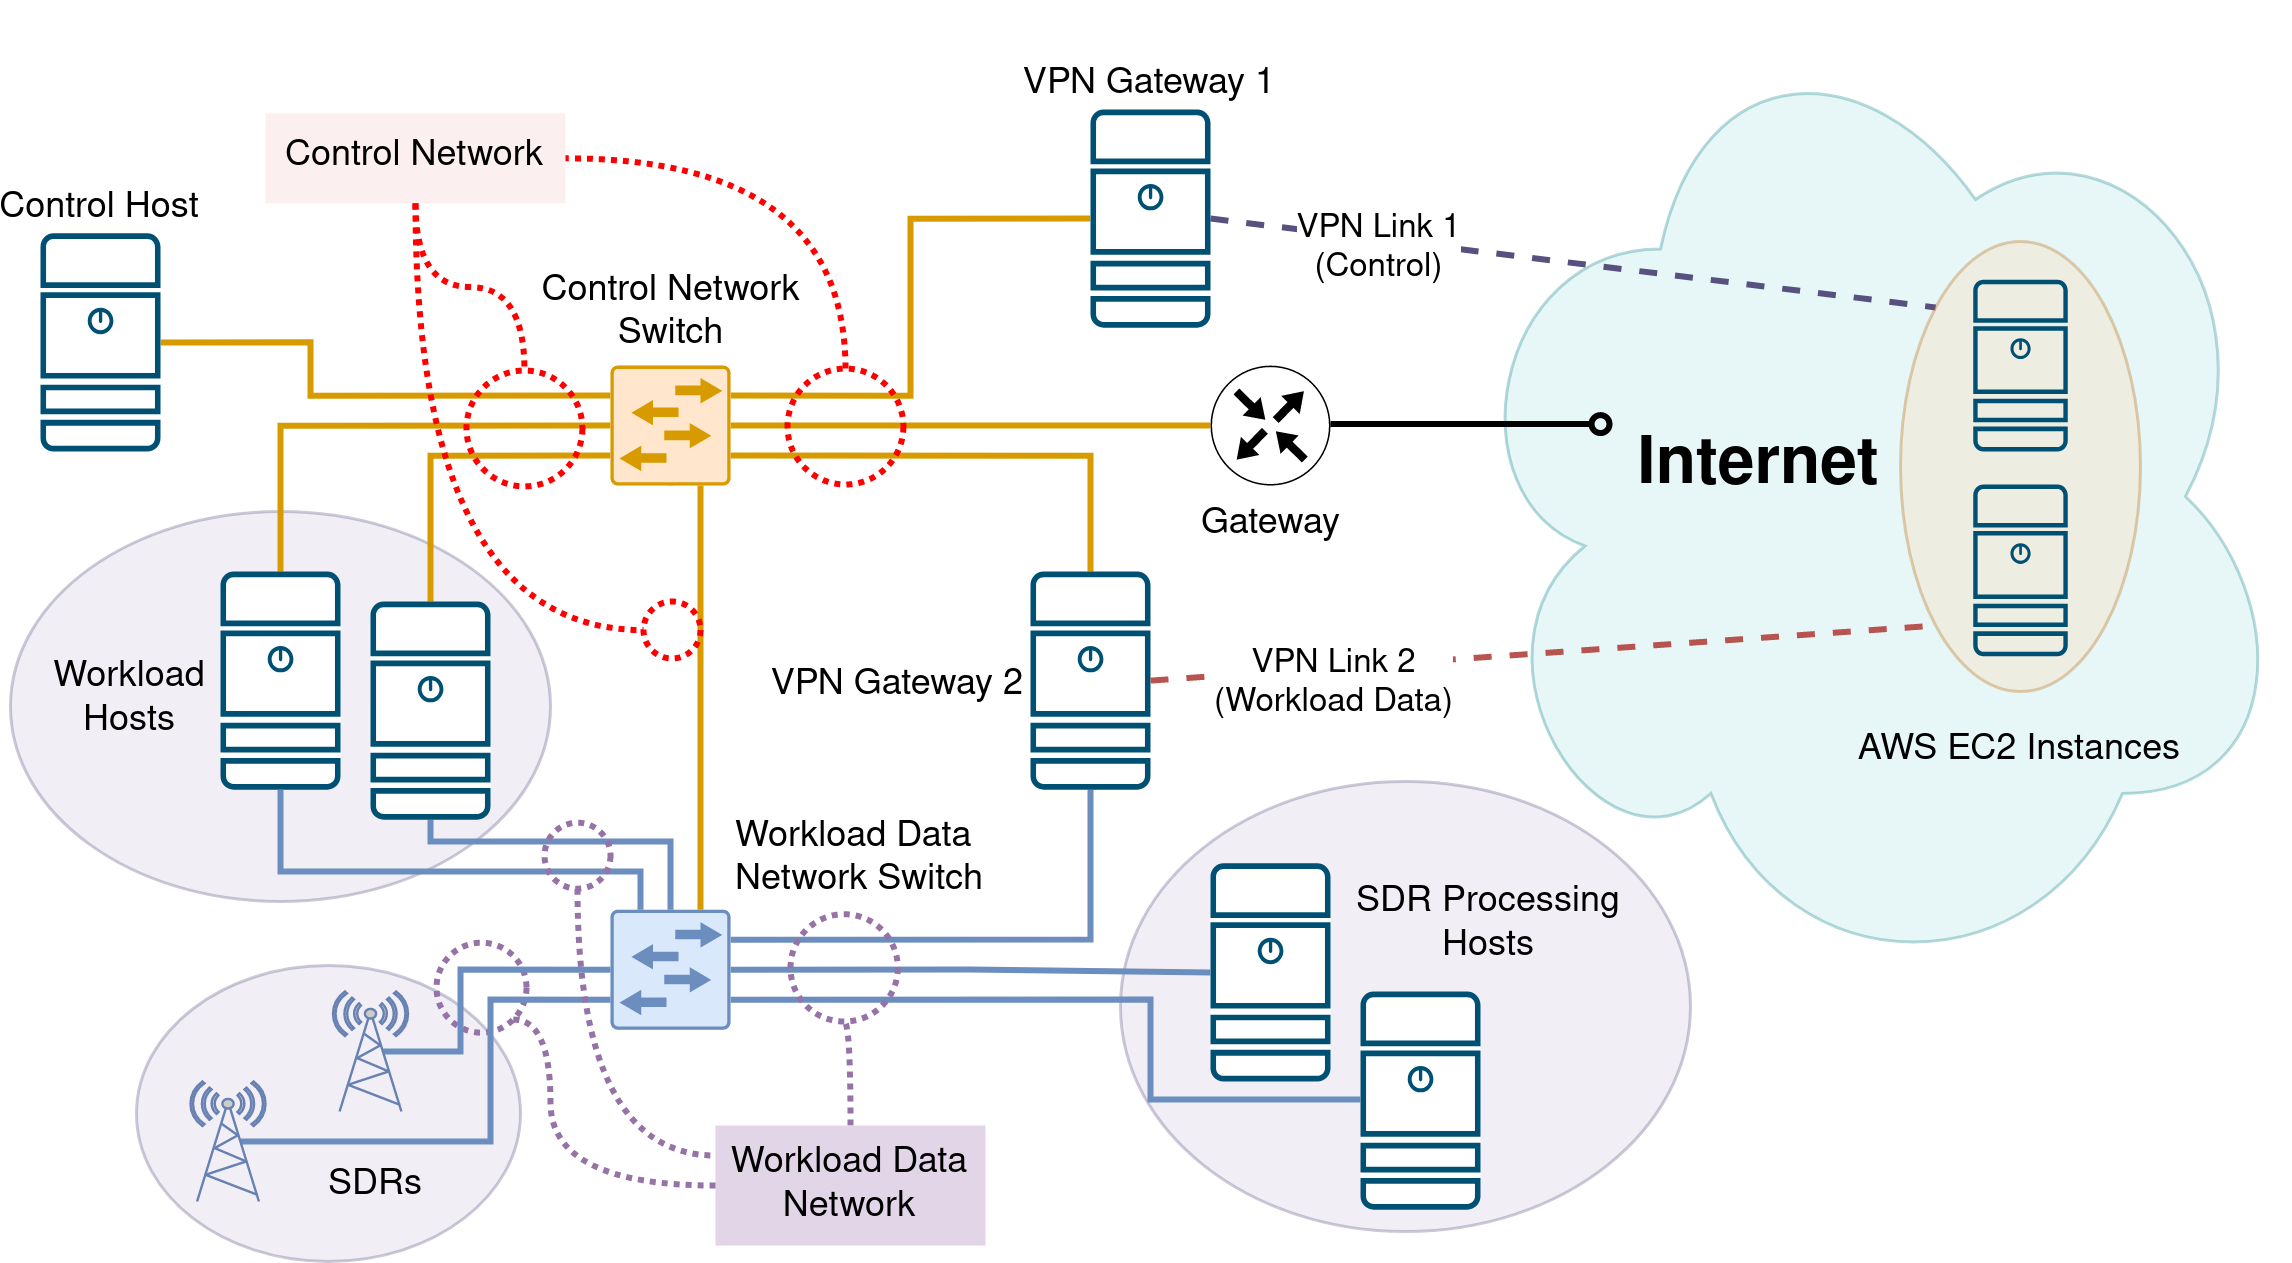
\includegraphics[width=.8\textwidth]{publications/2022Ainur/figures/network.png}
    \caption{Network structure assumed by Ainur.}\label{fig:network}
\end{figure*}